\section{Durchführung}
\label{sec:Durchführung}
\subsection{Kennlinien und Sättigungsstrom}
Zur Bestimmung der Kennlinien wird ein Aufbau wie in Abbildung \ref{fig:aufbaua} benutzt.
\begin{figure}
    \centering
    \caption{Schaltung zur Aufnahme der Diodenkennlinien \cite{v504}}
    \label{fig:aufbaua}
    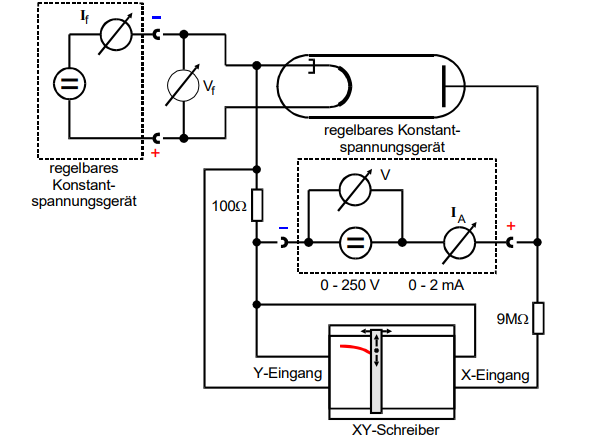
\includegraphics[width = 0.5 \textwidth]{pics/Aufbaua.png}
\end{figure}
Die Kennlinien werden durch Variation der Spannung zwischen Anode und Kathode entnommen. Dabei wird für jede neue Kennlinie der Heizstrom um $\SI{0.1}{\ampere}$ erhöht.
Die dazugehörigen Messwerte und Heizspannungen sind in Tabelle \ref{tab:charcurve} aufgeführt. 
An Stelle eines XY-Schreibers wird an einem Amperemeter der Diodenstrom $I_\text{A}$ abgelesen.
Aus den Messwerten lässt sich auch auf den Sättigungsstrom schließen.

\subsection{Anlaufstrom und Austrittsarbeit}
Die Messaperatur wird wie in Abbildung \ref{fig:aufbauc} aufgebaut.
\begin{figure}
    \centering
    \caption{Schaltung zur Aufnahme des Anlaufstroms \cite{v504}}
    \label{fig:aufbauc}
    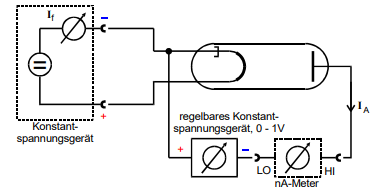
\includegraphics[width = 0.5 \textwidth]{pics/Aufbauc.png}
\end{figure}
Wesentliche Unterschiede zu dem Aufbau \ref{fig:aufbaua} sind dabei nur die Umpolung des Spannungsgerätes und das Austauschen des Amperemeters mit einem empfindlicheren Nanoamperemeter. Durch den eingebauten Verstärker ist dieses Gerät jedoch störungsanfälliger.
Bei der Messung wird der Heizstrom auf \SI{2.5}{\ampere} eingestellt und die Gegenspannung langsam hochskaliert. Die Messwerte werden an dem Amperemeter mit zugehöriger Gegenspannungen abgelesen.
